\chapter{Estado del arte} \label{sec:cap2}

\noindent El estudio del movimiento del cuerpo humano es una tarea compleja, que requiere de amplios conocimientos en el sector de la biomecánica, y herramientas específicas para su análisis. En este sentido, el sistema de captura de movimiento, conocido como \ac{MoCap}, es una herramienta fundamental para el estudio del movimiento humano \autocite{taiQueEsMotion2024}.

Durante este capítulo se presenta el estado del arte de la tecnología de captura de movimiento, y se analizan las diferentes herramientas que existen en el mercado para la visualización de los datos obtenidos. A continuación, se presenta el formato de fichero \ac{C3D}, que es el formato utilizado para almacenar los datos obtenidos por el sistema de captura de movimiento. Por último, se presentan los diferentes lenguajes de programación valorados para el desarrollo del proyecto, y se justifica la elección del mismo.

\section{Sistemas \textit{Motion Capture}}
El \textit{Motion Capture} es una técnica que permite capturar el movimiento de un objeto en tiempo real, y representarlo en un entorno virtual. Esta técnica se utiliza en diferentes campos, como la animación, la medicina, la biomecánica o la robótica; y se basa en la captura de la posición de diferentes marcadores en el espacio. Para lograr la captura, existen diferentes tecnologías, como cámaras de vídeo, sensores inerciales, sensores de ultrasonidos, etc. \autocite{taiQueEsMotion2024}

\subsection{\textit{Hardware} disponible}
En la facultad de \ac{INEF} de la \ac{UPM}, se utiliza un sistema de Motion Capture basado en cámaras de infrarrojo, que utilizan para capturar movimientos deportivos\footnote{La facultad de INEF cuenta con 6 cámaras infrarrojas de la marca Vicon, capaces de capturar fotogramas a una frecuencia de hasta 500 \ac{Hz} \autocite{FacultadCienciasActividad}}. Estos marcadores se colocan en diferentes partes del cuerpo del deportista, logrando capturar un movimiento preciso. Los datos capturados se almacenan en un fichero en formato \ac{C3D}, que contiene la información necesaria para la representación del movimiento.

Las tecnologías que existen en el mercado para la visualización de estos movimientos son muy costosas, y no siempre se adaptan a las necesidades de los investigadores. Por ello, en este proyecto se ha desarrollado una aplicación para la visualización de movimientos capturados en formato \ac{C3D}. La aplicación permite la visualización de los movimientos en un entorno tridimensional, pudiendo variar diferentes parámetros de la visualización, como la velocidad de reproducción, la posición de la cámara, la representación de los marcadores, de las uniones, vectores o fuerzas.

Es relevante señalar que este Proyecto se ciñe al sistema \ac{MoCap} disponible en la facultad de INEF de la \ac{UPM}, por el elevado coste de estos sistemas y la imposibilidad de trabajar con alternativas de la competencia. Sin embargo, existen otras alternativas con gran aceptación en el mercado. 

Se muestra en la \autoref{fig:laboratorio} el laboratorio de biomecánica de la facultad de \ac{INEF}, donde se pueden observar las cámaras Vicon, que son las utilizadas para la captura de movimiento. Este laboratorio está equipado con diferentes herramientas para el estudio del movimiento humano, como plataformas de fuerza, sistemas de captura de movimiento, etc.

\begin{figure}[H]
    \centering
    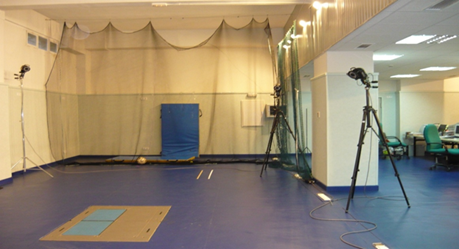
\includegraphics[width=\textwidth]{laboratorio biomecanica.png}
    \caption{Laboratorio de biomecánica de la facultad de \ac{INEF}.}
    \label{fig:laboratorio}
\end{figure}

\subsection{Alternativas}
Existen diferentes alternativas a los sistemas Vicon disponibles en el mercado, como los sistemas OptiTrack o Qualisys. En el artículo \autocite{article} se comparan estos sistemas, quedando patente que estos sistemas son capaces de capturar correctamente el movimiento. Además, en la \autoref{fig:errores-mocap} se aprecia como los errores de estos sistemas se han ido reduciendo a lo largo del tiempo.

\begin{figure}[H]
    \centering
    \includegraphics[width=\textwidth]{errores-mocap.png}
    \caption{Error absoluto de diferentes sistemas. Obtenido de \autocite{article}.}
    \label{fig:errores-mocap}
\end{figure}

\section{Ficheros \acs{C3D}} \label{sec:ficheros-c3d}
Entender el formato de los ficheros \ac{C3D} es fundamental para el desarrollo de esta aplicación. 

El formato \ac{C3D} es un formato de fichero binario de dominio público que se crea a mediados de los años 80, en el \textit{National Institutes of Health Biomechanics Laboratory}, en Maryland, USA, y es compatible con todos los principales sistemas de captura de movimiento 3D. Es usado por empresas de las industrias de biomecánica, captura de movimiento y animación \autocite{C3DORGBiomechanicsStandard}.

Un fichero \ac{C3D} es un fichero binario que contiene toda la información de la captura de movimiento. Como se explica en \autocite{C3DORGBiomechanicsStandard}, este fichero se compone de diferentes secciones, que contienen la información de los marcadores para cada fotograma de la captura. Se utilizan estos ficheros en vez de ficheros de texto para reducir el tamaño del fichero, y para garantizar la integridad de los datos.

Es importante señalar que el formato \ac{C3D} contiene información de objetos con coordenadas tridimensionales, pero estos objetos no tienen por qué ser marcadores. Por ejemplo, en el fichero \ac{C3D} se pueden almacenar diferentes tipos de objetos, como marcadores, vectores, fuerzas, etc. Por tanto, es importante entender el formato \ac{C3D} para poder extraer la información necesaria para la representación del movimiento. Además, es necesaria una herramienta para filtrar la información que se quiere representar, ya que un fichero \ac{C3D} puede contener miles de objetos, y no todos ellos son relevantes para la representación del movimiento.

Existen diferentes \textit{parsers} que permiten la lectura de estos ficheros, y la extracción de la información necesaria para la representación del movimiento. En este proyecto se ha modificado el \textit{crate} \texttt{c3dio}, que permite la lectura de ficheros \ac{C3D} en Rust, y tiene un \textit{plugin} para \texttt{Bevy} que facilita la integración con el motor de videojuegos, que se explica en el \autoref{subsec:bevy}. Adicionalmente, con la herramienta explicada en el \autoref{apx:c3d_latex_py}, se puede convertir un fragmento de un fichero \ac{C3D} a un formato leíble por humanos. Se muestra en la \autoref{tab:c3d_data} un fragmento de un fichero \ac{C3D} utilizado durante el desarrollo de la aplicación, que contiene información sobre los primeros diez fotogramas de la captura de movimiento, para dos marcadores, \ac{RFIN} y \ac{RFRA}.

\begin{table}[htbp]
    \centering
    \setlength{\tabcolsep}{5pt}
    \renewcommand{\arraystretch}{1.2}
    \rowcolors{3}{white}{gray!10}
    \begin{tabular}{r|S[table-format=-3.2]S[table-format=-3.2]S[table-format=-3.2]|S[table-format=-3.2]S[table-format=-3.2]S[table-format=-3.2]}
    \toprule
    \multirow{2}{*}{\textbf{Frame}} & \multicolumn{3}{c|}{RFIN                          } & \multicolumn{3}{c}{RFRA                          } \\
      & {\textbf{x}} & {\textbf{y}} & {\textbf{z}} & {\textbf{x}} & {\textbf{y}} & {\textbf{z}} \\
    \midrule
    1 & 46.80 & 3.25 & 664.41 & -23.14 & -4.06 & 827.33 \\
    2 & 46.80 & 3.25 & 664.41 & -23.14 & -4.07 & 827.30 \\
    3 & 46.80 & 3.25 & 664.41 & -23.14 & -4.08 & 827.30 \\
    4 & 46.80 & 3.25 & 664.41 & -23.14 & -4.07 & 827.30 \\
    5 & 46.80 & 3.25 & 664.41 & -23.15 & -4.06 & 827.31 \\
    \midrule
    6 & 46.80 & 3.25 & 664.41 & -23.16 & -4.03 & 827.33 \\
    7 & 46.81 & 3.25 & 664.41 & -23.18 & -4.00 & 827.35 \\
    8 & 46.82 & 3.28 & 664.40 & -23.21 & -3.99 & 827.36 \\
    9 & 46.87 & 3.36 & 664.40 & -23.23 & -4.02 & 827.33 \\
    10 & 46.93 & 3.51 & 664.38 & -23.23 & -4.09 & 827.26 \\
    \bottomrule
    \end{tabular}
    \caption{Fragmento de un fichero \acs{C3D} convertido a tabla}
    \label{tab:c3d_data}
\end{table}
  
Se puede observar que aparecen los dos marcadores mencionados, junto con sus coordenadas en el espacio, representadas por los valores de las columnas \textit{x}, \textit{y} y \textit{z}, en unidades de milímetros.

\subsection{Herramientas actuales para la visualización de ficheros \acs{C3D}}

Las herramientas actuales que existen en el mercado para la visualización de un fichero \ac{C3D} son escasas y generalmente costosas. Una biblioteca famosa en el pasado para el tratamiento de ficheros \ac{C3D} era la \textit{Biomechanics ToolKit} - BTK, pero fue comprada por la compañía canadiense \textit{Movec}, que tiene intención de renovarla bajo el nombre comercial \textit{Bridge} \autocite{Bridge,ProjectBiomechanicalToolKit}. Por otro lado, el entorno de trabajo proporcionado por las cámaras Vicon de \ac{INEF} es antiguo y tosco, no admitiendo características clave en el la época actual, como la visualización en línea. Además, su licencia es propietaria y tiene un coste elevado.

Se muestra en la \autoref{fig:entorno-vicon} el entorno de trabajo actual con el que cuenta la facultad de \ac{INEF}, donde se aprecia que el entorno está desfasado. Además, las opciones de personalización son escasas, limitándose a la selección de marcadores y a la visualización de los mismos.

\begin{figure}[H]
    \centering
    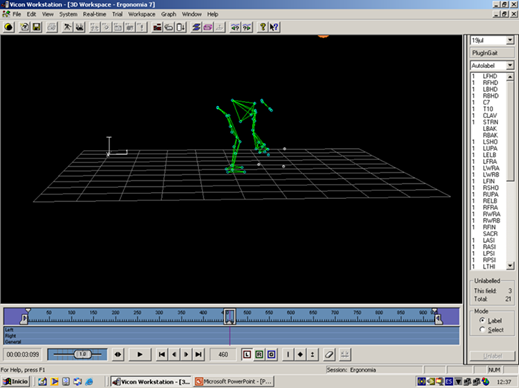
\includegraphics[width=\textwidth]{entorno enrique.png}
    \caption{Entorno actual de Vicon}
    \label{fig:entorno-vicon}
\end{figure}

\section{Lenguaje de programación}

Un aspecto importante para este proyecto es la elección del lenguaje de programación. Al ser un proyecto que no hereda de ningún otro, hay libertad para elegir el lenguaje de programación que se considere más adecuado. Sin embargo, elegir un buen lenguaje de programación es fundamental para el éxito del proyecto, ya que un lenguaje de programación inadecuado puede hacer que el proyecto sea difícil de mantener y de escalar.

Como se explica en el \autoref{sec:ficheros-c3d}, un fichero \ac{C3D} contiene toda la información de la posición de los marcadores a lo largo de la grabación del movimiento. Una frecuencia de muestreo típica en este tipo de ficheros es de 250 \ac{Hz}, lo que significa que se captura la posición de los marcadores 250 veces por segundo. Adicionalmente, al fichero \ac{C3D} se le añaden puntos calculados, que pueden ser articulaciones entre dos marcadores reales, vectores de velocidad, aceleraciones, etc. Por tanto, es común que un fichero \ac{C3D} contenga miles de puntos, lo que hace que la visualización de estos movimientos sea una tarea compleja y exigente en términos de rendimiento.

Adicionalmente, en el planteamiento del proyecto, se especificó que debían existir dos versiones, una de escritorio y una versión web, bajo el mismo código fuente. Esto implica que el mismo código fuente debe poder ser compilado a los sistemas operativos mayoritarios, y además debe poder ser ejecutada en un entorno web. Con estas premisas, se han valorado diferentes lenguajes de programación para el desarrollo de la aplicación.  

\subsection{JavaScript}
JavaScript es un lenguaje de programación interpretado, que se ha convertido en el estándar para el desarrollo de aplicaciones web. Este lenguaje está muy optimizado, gracias a avances en los motores de JavaScript, como SpiderMonkey de Mozilla o V8 de Google \autocite{srinetChromeV8Firefox2022}. Para el desarrollo de aplicaciones de escritorio, JavaScript se puede utilizar con diferentes tecnologías, como Electron \autocite{BuildCrossplatformDesktop}, que permite la creación de aplicaciones de escritorio multiplataforma con tecnologías web. 

Pese a esto, el mayor problema de JavaScript es el rendimiento, ya que este lenguaje no dispone de características de bajo nivel, como la gestión de memoria o la programación concurrente \autocite{MemoryManagementJavaScript2025,pengMultithreadingJavascript2017}. Por tanto, JavaScript no es un lenguaje de programación adecuado para el desarrollo de aplicaciones que requieren un alto rendimiento, como es el caso de la visualización de movimientos en 3D.

\subsection{Python}
Python es un lenguaje de programación interpretado, que se ha convertido en uno de los lenguajes de programación más populares en la actualidad \autocite{TIOBEIndex}. Python es un lenguaje de programación de tipado dinámico, que permite la inferencia de tipos, y que garantiza la seguridad de la memoria en tiempo de ejecución. Este lenguaje de programación resulta muy versátil, utilizándose en diferentes campos, como la inteligencia artificial, el análisis de datos, la programación web, etc. Además, dispone de una gran cantidad de bibliotecas y \textit{frameworks}, que facilitan el desarrollo de aplicaciones de todo tipo.

Sin embargo, al igual que JavaScript, Python no es un lenguaje de programación especialmente rápido, ya que es un lenguaje interpretado, y generalmente sus bibliotecas son pesadas y poco eficientes, por lo que se suele considerar un lenguaje ideal únicamente para prototipado \autocite{SlowestProgrammingLanguages2020}.

\subsection{C++}
C++ es un lenguaje de programación de propósito general, que se utiliza en diferentes campos, como la programación de sistemas, la programación de videojuegos, la programación de aplicaciones de escritorio, etc. C++ es un lenguaje de programación de tipado estático, que permite la inferencia de tipos, y que garantiza la seguridad de la memoria en tiempo de compilación. C++ es un lenguaje de programación muy eficiente, que permite la programación de bajo nivel, y que dispone de una gran cantidad de bibliotecas y frameworks, que facilitan el desarrollo de aplicaciones de todo tipo. C++ es un lenguaje de programación muy rápido, que se utiliza en aplicaciones que requieren un alto rendimiento, como videojuegos, motores de renderizado o sistemas operativos, entre otros. 

Sin embargo, C++ es un lenguaje de programación antiguo, que no dispone de características modernas, como un gestor de paquetes para la gestión de dependencias. Además, C++ no es un lenguaje de programación concebido para el desarrollo de aplicaciones web, y si bien existen herramientas para compilar C++ a \textit{WebAssembly}, su uso no es mayoritario.

\subsection{Rust}
El lenguaje de programación Rust es un lenguaje de programación innovador que prioriza la seguridad y la eficiencia. Este lenguaje ha sido diseñado por Mozilla Research, y se ha convertido en uno de los lenguajes de programación más populares en la actualidad. Rust es un lenguaje de programación multiparadigma, que combina elementos de programación funcional, orientada a objetos e imperativa. Este es un lenguaje de programación de tipado estático, que permite la inferencia de tipos, y que garantiza la seguridad de la memoria en tiempo de compilación.

Rust dispone de características modernas, como un gestor de paquetes para la gestión de dependencias, llamado Cargo, y compilación nativa a WebAssembly, lo que permite la ejecución de código Rust en un navegador web \autocite{WebAssembly}. Por tanto, cumple los objetivos del proyecto, al permitir la compilación a los sistemas operativos mayoritarios, y a un entorno web.

\subsubsection{WebAssembly y wasm-bindgen}

WebAssembly (WASM) es un formato binario de bajo nivel diseñado como destino de compilación para lenguajes de alto nivel, permitiendo ejecutar código con un rendimiento cercano al nativo en navegadores web \autocite{WebAssembly}. Rust es uno de los lenguajes con mejor soporte para WASM, gracias a su sistema de tipos y gestión de memoria sin recolector de basura.

La herramienta \texttt{wasm-bindgen} \autocite{IntroductionWasmbindgenGuide} facilita la interoperabilidad entre Rust y JavaScript, permitiendo el intercambio de datos complejos entre ambos lenguajes. Esta biblioteca automatiza gran parte del trabajo necesario para la comunicación entre el código Rust compilado a WASM y el entorno JavaScript del navegador, resolviendo una de las limitaciones mencionadas anteriormente: la falta de acceso directo al DOM.

Con \texttt{wasm-bindgen}, es posible exponer funciones Rust a JavaScript y viceversa, trabajar con tipos de JavaScript desde Rust, y manipular el DOM a través de interfaces que resultan naturales para los programadores de Rust. Esto hace que el desarrollo de aplicaciones web con Rust sea una alternativa viable y eficiente a JavaScript puro, especialmente para componentes que requieren alto rendimiento o seguridad de memoria.

\subsection{Otras herramientas consideradas}
\subsubsection{Unity}
Unity es un motor de videojuegos multiplataforma, que permite el desarrollo de videojuegos en 2D y 3D. Este motor se puede utilizar también como herramienta para crear simulaciones, que es el propósito de este proyecto. Unity dispone de una gran cantidad de herramientas y bibliotecas, que facilitan el desarrollo de aplicaciones de todo tipo. Sin embargo, Unity es un motor de videojuegos pesado, que consume muchos recursos, y que no es especialmente eficiente en términos de rendimiento, sobre todo en entornos web.

\subsection{Comparativa de rendimiento}

Como se puede observar en la \autoref{fig:comparativa-rendimiento}, que coincide con el análisis publicado en \textit{Medium} \autocite{samTop10Fastest2024}, Rust cae en los primeros puestos por rendimiento, teniendo un rendimiento similar al de C y C++, y superando ampliamente a Python y Node.js (\textit{JavaScript}).

\begin{figure}[H]
    \centering
    \includegraphics[width=\textwidth]{comparativa rendimiento lenguajes.png}
    \caption{Comparativa de rendimiento en entornos de escritorio \autocite{zotero-253}}
    \label{fig:comparativa-rendimiento}
\end{figure}

% https://goodmanwen.github.io/Programming-Language-Benchmarks-Visualization/

Sin embargo, esta tabla no es válida en entornos web, dado que en estos entornos el rendimiento de los diferentes lenguajes de programación se ve limitado por características propias de los navegadores. Por ejemplo, Rust compilado a WebAssembly no tiene acceso directo al \ac{DOM}, que es el modelo de objetos de un documento HTML. Esto significa que Rust no puede manipular directamente los elementos de la página web, y que necesita comunicarse con JavaScript para hacerlo. 

Un \textit{benchmark} de rendimiento en entornos web se puede encontrar en \autocite{InteractiveResults}, que muestra que \textit{vanilla JavaScript} es el lenguaje más rápido en este tipo de entornos. Sin embargo, en un proyecto como este, no se contempla el uso de \textit{vanilla JavaScript}, puesto que se necesita un \textit{framework} que permita la creación de aplicaciones gráficas de forma sencilla y eficiente. Si se analiza el rendimiento de diferentes \textit{frameworks} en entornos web, se puede ver que la diferencia entre los basados en \textit{JavaScript} y los basados en \textit{Rust} es mínima, no habiendo un claro vencedor en este aspecto \autocite{InteractiveResults}.

\subsection{Elección del lenguaje de programación}

Valorando las diferentes opciones, se ha decidido utilizar Rust para el desarrollo de la aplicación. Las características que han sido determinantes en la elección de Rust son las siguientes:

\begin{enumerate}
    \item \textbf{Seguridad:} Rust es un lenguaje de programación que garantiza la seguridad de la memoria en tiempo de compilación, lo que evita errores comunes en la programación, como los desbordamientos de búfer o las fugas de memoria.
    \item \textbf{Eficiencia:} Rust es un lenguaje de programación muy eficiente, que permite la programación de bajo nivel, y que garantiza un alto rendimiento en la ejecución del código.
    \item \textbf{Modernidad:} Rust es un lenguaje de programación moderno, que dispone de características avanzadas, como un gestor de paquetes para la gestión de dependencias, y compilación nativa a WebAssembly.
    \item \textbf{Versatilidad:} Rust es un lenguaje de programación multiparadigma, que combina elementos de programación funcional, orientada a objetos e imperativa, lo que facilita el desarrollo de aplicaciones de todo tipo.
\end{enumerate}

\section{Ficheros de configuración} \label{sec:ficheros-configuracion}

Los ficheros \ac{C3D} que este proyecto pretende representar pueden tener un número muy elevado de marcadores, superando ampliamente el millar. Representar una cantidad muy elevada de marcadores en el entorno es contraproducente, pues no permite focalizar en los puntos que se pretende estudiar. Por tanto, es importante generar una configuración que permita seleccionar los marcadores de interés.

Vicon cuenta con un formato propietario para definir configuraciones que su aplicación de representación de movimiento utiliza. En el \autoref{lst:mkr} se muestra un fragmento de este tipo de ficheros, (formato MKR), que presenta una única configuración de marcadores, llamada \texttt{Autolabel}.

\begin{lstlisting}[style=mystyle, caption={Fragmento de un fichero MKR}, label=lst:mkr]
!MKR#2

[Autolabel]
	LFHD	Left front head
	RFHD	Right front head
	LBHD	Left back head
	RBHD	Right back head

    LFHD,RFHD,LBHD,RBHD
\end{lstlisting}

En esta configuración, se definen cuatro marcadores, \texttt{LFHD}, \texttt{RFHD}, \texttt{LBHD} y \texttt{RBHD}, y se les añade una breve descripción. Estos marcadores serán los que la aplicación represente. En la última línea se especifica que estos marcadores se unirán con una línea, por estar separados mediante comas. Este formato es sencillo y fácil de entender, pero no es demasiado flexible, y no permite variar el tamaño, forma o color de los marcadores o uniones.

Para este proyecto, se ha decidido usar un formato estándar, con un mayor número de opciones que el formato MKR. Para este caso de uso existen diversos lenguajes de configuración comúnmente utilizados.

\subsection{\acs{JSON}}

\ac{JSON} es un formato de serialización de datos ligero y de fácil lectura para humanos y máquinas. Originalmente derivado de JavaScript, \ac{JSON} es un fichero comúnmente utilizado en numerosos entornos por su simplicidad.

Este formato utiliza una estructura basada en pares clave-valor y soporta tipos de datos básicos como números, cadenas de texto, booleanos, listas y objetos anidados. Su sintaxis compacta y la amplia disponibilidad de bibliotecas para su procesamiento en prácticamente todos los lenguajes de programación lo han convertido en una opción popular para la configuración de aplicaciones e intercambio de datos \autocite{ECMA404}.

A pesar de su popularidad, \ac{JSON} presenta algunas limitaciones como la falta de soporte nativo para comentarios y la necesidad de utilizar comillas para las claves, lo que puede reducir su legibilidad en configuraciones complejas.

\subsection{\acs{YAML}}

Igual que \ac{JSON}, \ac{YAML} es un formato de serialización de datos que se utiliza comúnmente para la configuración y el intercambio de datos. Sin embargo, \ac{YAML} se diseñó con un enfoque en la legibilidad humana, utilizando sangría para definir la estructura jerárquica en lugar de llaves y corchetes.

Este formato destaca por su sintaxis minimalista que elimina la mayoría de los símbolos de puntuación y permite representar datos complejos de manera clara. \ac{YAML} soporta todos los tipos de datos básicos de \ac{JSON}, pero añade características adicionales como soporte nativo para comentarios, referencias y etiquetas de tipo explícitas \autocite{YAMLAintMarkup}.

Una de las ventajas principales de \ac{YAML} es su capacidad para representar configuraciones complejas de manera concisa y legible. Es ampliamente utilizado en herramientas de infraestructura como código, configuración de aplicaciones y plataformas de contenedores como Docker y Kubernetes \autocite{FicheroDockercomposeyml,february2024YAMLBasicsKubernetes}.

Sin embargo, \ac{YAML} también presenta algunos inconvenientes, como la dependencia en la sangría que puede generar errores difíciles de detectar, y una sintaxis que en ocasiones puede resultar ambigua, especialmente en el manejo de cadenas de texto con caracteres especiales.

\subsection{\acs{TOML}}

\ac{TOML} es un formato de serialización de datos diseñado para ser un lenguaje de configuración sencillo y legible. \ac{TOML} es famoso por su uso en Rust, siendo el formato oficial para los ficheros de configuración \texttt{Cargo.toml} del gestor de paquetes de Rust.

Este formato se caracteriza por su sintaxis clara que recuerda a los ficheros INI pero con tipos de datos más ricos y soporte para estructuras jerárquicas. \ac{TOML} destaca por su capacidad para representar datos complejos de manera clara y sin ambigüedades, lo que lo hace ideal para configuraciones de aplicaciones \autocite{TOMLEnglishV100}.

\subsection{Elección del formato de configuración}

En este proyecto se ha decidido utilizar el formato \ac{TOML} para definir la configuración de representación. Este formato es sencillo y comparte similitudes con el formato MKR de Vicon. Además, \ac{TOML} es un formato de configuración ampliamente utilizado en el ecosistema de Rust, lo que da visibilidad a este lenguaje.

\section{Herramientas de desarrollo}

En este apartado se desarrollan las diferentes herramientas que se han utilizado para el desarrollo de la aplicación. Debido a la naturaleza del proyecto, se ha decidido utilizar un motor de videojuegos para abstraer la complejidad de la representación gráfica. Sobre este motor se han integrado diferentes herramientas, como un \textit{parser} para ficheros \ac{C3D}, y un sistema de configuración para la representación del mismo.

% Para conseguir una aplicación gráfica eficiente, se debe de contar con una interfaz que permita a la aplicación trabajar con el hardware del dispositivo. Por tanto, es importante utilizar herramientas multiplataforma que permitan a la aplicación ser eficiente en diferentes entornos. En Rust, existen muchos \textit{crates} (unidades de compilación, ver \autocite{PackagesCratesRust}) que permiten el desarrollo de aplicaciones gráficas, como \texttt{wgpu} \autocite{WgpuPortableGraphics}, \texttt{glium} \autocite{GliumGlium2025}, \texttt{piston} \autocite{PistonModularOpen}, etc. Sin embargo, estos \textit{crates} son de muy bajo nivel, y crear una aplicación gráfica desde cero con ellos puede ser una tarea exigente en términos de tiempo. 

\subsection{Bevy} \label{subsec:bevy}
Como motor de videojuegos, se ha decidido utilizar \textit{Bevy}, que se caracteriza por su enfoque modular, e implemente internamente diferentes APIs gráficas, abstrayendo la complejidad de lidiar con ellas y haciendo a la aplicación multiplataforma. \textit{Bevy}, que está escrito plenamente en Rust y que cuenta con una comunidad numerosa y activa \autocite{BevyEngine}.

Las principales características de \texttt{Bevy} son las siguientes:
\begin{enumerate}
    \item \textbf{Eficiencia:} \texttt{Bevy} es un motor de videojuegos muy eficiente, que garantiza un alto rendimiento en la ejecución del código. Consigue esta eficiencia gracias a su diseño modular, que implica que sólo se compilarán los módulos del motor que el proyecto necesite. Utiliza programación concurrente siempre que es posible (esta es una limitación importante de los entornos web), y dispone de un sistema de eventos que permite la comunicación entre diferentes sistemas.
    \item \textbf{Soporte multiplataforma:} Como se ha comentado, \texttt{Bevy} es un motor de videojuegos multiplataforma, que interacciona con diferentes APIs gráficas, como Vulkan, Metal o DirectX en entornos de escritorio, o WebGPU en entornos web. Esto permite que una aplicación desarrollada con \texttt{Bevy} pueda ejecutarse en diferentes sistemas operativos, como Windows, macOS, Linux o la web. La elección de la API gráfica se realiza de forma automática, en función del sistema operativo en el que se ejecute la aplicación.
\end{enumerate}

Otro aspecto destacado de \texttt{Bevy} es que se basa en el patrón de diseño ECS (\textit{Entity-Component-System}), que permite la creación de entidades, componentes y sistemas de forma independiente. 

La versión que este proyecto utiliza de \texttt{Bevy} es la 0.15.0, que fue la versión más reciente al momento de la implementación del proyecto.

\subsubsection{Paradigma \acs{ECS}} \label{subsec:ecs}

El paradigma \ac{ECS} es un patrón arquitectónico de software que ha ganado popularidad en el desarrollo de videojuegos y simulaciones por su eficiencia y flexibilidad \autocite{prdevingDeepdivingEntityComponent2023}. Diferentes artículos, como \autocite{zaksWhenNotUse2018} mencionan que este patrón es especialmente útil para aplicaciones interactivas.

A diferencia de los patrones tradicionales orientados a objetos, \ac{ECS} descompone la lógica de la aplicación en tres elementos principales \autocite{SistemaComponentesEntidad2024}:

\begin{itemize}
    \item \textbf{Entidades:} Son identificadores únicos que representan objetos en el mundo virtual. En sí mismas, las entidades no contienen datos ni comportamiento, funcionando más bien como contenedores lógicos para componentes.
    
    \item \textbf{Componentes:} Son estructuras de datos puras que contienen solo propiedades, sin comportamiento asociado. Cada componente representa un aspecto específico de una entidad (posición, renderizado, física, etc.). Una entidad puede tener múltiples componentes, siguiendo el principio de composición sobre herencia.
    
    \item \textbf{Sistemas:} Contienen la lógica que procesa entidades con combinaciones específicas de componentes. Cada sistema opera sobre un conjunto de componentes de forma independiente, realizando transformaciones en los datos.
\end{itemize}

En el contexto de Bevy, el paradigma \ac{ECS} se implementa de manera eficiente mediante un concepto adicional: los \textit{recursos}. Estos son datos globales accesibles por los sistemas sin estar asociados a entidades específicas. \textit{Bevy} también implementa un sistema de eventos que permite la comunicación entre sistemas sin acoplarlos directamente.

\subsection{EGUI} \label{subsec:egui}

Las aplicaciones de escritorio suelen implementar una \ac{GUI} que permite al usuario interactuar con la aplicación. Los \textit{frameworks} más utilizados para la creación de una \ac{GUI} son Qt \autocite{Theqtstory}, que se ha usado para crear aplicaciones famosas como el popular reproductor de vídeo y música VLC \autocite{QtGTKVideoLAN}, o GTK, que es el \textit{framework} utilizado por el entorno de escritorio GNOME, o el editor de fotografías GIMP. 

Pese a que estos \textit{frameworks} están escritos en C/C++, tienen \textit{bindings} a otros lenguajes de programación, como Rust. Sin embargo, para este proyecto se ha decidido utilizar un motor de videojuegos para facilitar el cálculo de la física y la representación gráfica. Por tanto, se ha decidido utilizar un \textit{framework} de \ac{GUI} que esté escrito en Rust y que sea compatible con \texttt{Bevy}. 

Un ejemplo de este tipo de \textit{frameworks} es \texttt{egui}, que es una biblioteca gráfica escrita en Rust, y que dispone compilación nativa a WebAssembly. Así, la misma \ac{GUI} es válida tanto para la aplicación de escritorio como para la versión web \autocite{ernerfeldtEmilkEgui2025}.

Adicionalmente, existe una adaptación de \texttt{egui} para \texttt{Bevy}, que permite la integración de la \ac{GUI} con el motor de videojuegos. Esta adaptación se llama \texttt{bevy\_egui} \autocite{Bevy_eguiRust}. 

\subsection{Arquitectura orientada a eventos} \label{subsec:eventos}

La arquitectura orientada a eventos es un patrón de diseño que organiza el flujo de un sistema en torno a la producción, detección y consumo de eventos, en lugar de seguir una secuencia lineal de instrucciones. Un evento representa un cambio en el estado del sistema o una señal externa que requiere atención \autocite{SistemaComponentesEntidad2024}.

En este patrón arquitectónico se identifican tres componentes principales:
\begin{itemize}
    \item \textbf{Emisores de eventos:} Entidades que generan y publican eventos cuando ocurre un cambio relevante en su estado o cuando detectan alguna condición específica.
    
    \item \textbf{Canales de eventos:} Infraestructura que permite transportar los eventos desde los emisores hasta los consumidores, pudiendo incluir colas, buses de eventos o mecanismos de publicación/suscripción.
    
    \item \textbf{Consumidores de eventos:} Componentes que reciben eventos y ejecutan lógica específica en respuesta a ellos, pudiendo a su vez generar nuevos eventos.
\end{itemize}

Esta arquitectura ofrece numerosas ventajas para aplicaciones interactivas, como:

\begin{itemize}
    \item \textbf{Acoplamiento débil:} Los emisores y consumidores de eventos no necesitan conocerse entre sí, lo que facilita el desarrollo y el mantenimiento de componentes individuales.
    
    \item \textbf{Escalabilidad:} Cada sistema puede reaccionar a múltiples eventos, siendo especialmente útil para aplicaciones con interfaces gráficas complejas o procesamiento asíncrono.
    
    \item \textbf{Reactividad:} Permite responder rápidamente a cambios en el estado de la aplicación o a acciones del usuario, relevante en los sistemas interactivos.
    
    \item \textbf{Extensibilidad:} Nuevas funcionalidades pueden añadirse creando nuevos consumidores de eventos existentes, sin modificar los componentes existentes.
\end{itemize}

\texttt{Bevy} implementa un sistema de eventos robusto que se integra perfectamente con su arquitectura \ac{ECS}. Los eventos en \texttt{Bevy} son estructuras de datos tipados que pueden ser enviados a través de un sistema de colas gestionado por el motor. Los sistemas pueden registrarse como receptores de tipos específicos de eventos y procesar solo aquellos relevantes para su funcionamiento \autocite{EventsBevyPrelude,EventsUnofficialBevy}. Esto permite una clara separación entre subsistemas mientras se mantiene un flujo de datos coherente.

% \subsection{Fundamentos de representación 3D}

% La representación tridimensional se basa en varios conceptos fundamentales. Las primitivas geométricas constituyen los elementos básicos utilizados para construir otros objetos complejos. Estos elementos se sitúan en sistemas de coordenadas cartesianas donde, por convenio, suele establecerse el eje Y vertical (contra la gravedad), aunque estas convenciones pueden variar entre diferentes aplicaciones.

% La manipulación espacial de estos elementos requiere transformaciones geométricas (traslación, rotación y escalado), esenciales para posicionar correctamente los elementos a lo largo del tiempo. La percepción visual de estos elementos se consigue mediante técnicas de iluminación y asignación de materiales, que determinan características como el color o brillo. La selección adecuada de estos atributos mejora la percepción de profundidad y facilita la distinción entre diferentes elementos.



